% Options for packages loaded elsewhere
\PassOptionsToPackage{unicode}{hyperref}
\PassOptionsToPackage{hyphens}{url}
%
\documentclass[
  man,floatsintext]{apa6}
\usepackage{amsmath,amssymb}
\usepackage{lmodern}
\usepackage{iftex}
\ifPDFTeX
  \usepackage[T1]{fontenc}
  \usepackage[utf8]{inputenc}
  \usepackage{textcomp} % provide euro and other symbols
\else % if luatex or xetex
  \usepackage{unicode-math}
  \defaultfontfeatures{Scale=MatchLowercase}
  \defaultfontfeatures[\rmfamily]{Ligatures=TeX,Scale=1}
\fi
% Use upquote if available, for straight quotes in verbatim environments
\IfFileExists{upquote.sty}{\usepackage{upquote}}{}
\IfFileExists{microtype.sty}{% use microtype if available
  \usepackage[]{microtype}
  \UseMicrotypeSet[protrusion]{basicmath} % disable protrusion for tt fonts
}{}
\makeatletter
\@ifundefined{KOMAClassName}{% if non-KOMA class
  \IfFileExists{parskip.sty}{%
    \usepackage{parskip}
  }{% else
    \setlength{\parindent}{0pt}
    \setlength{\parskip}{6pt plus 2pt minus 1pt}}
}{% if KOMA class
  \KOMAoptions{parskip=half}}
\makeatother
\usepackage{xcolor}
\usepackage{longtable,booktabs,array}
\usepackage{calc} % for calculating minipage widths
% Correct order of tables after \paragraph or \subparagraph
\usepackage{etoolbox}
\makeatletter
\patchcmd\longtable{\par}{\if@noskipsec\mbox{}\fi\par}{}{}
\makeatother
% Allow footnotes in longtable head/foot
\IfFileExists{footnotehyper.sty}{\usepackage{footnotehyper}}{\usepackage{footnote}}
\makesavenoteenv{longtable}
\usepackage{graphicx}
\makeatletter
\def\maxwidth{\ifdim\Gin@nat@width>\linewidth\linewidth\else\Gin@nat@width\fi}
\def\maxheight{\ifdim\Gin@nat@height>\textheight\textheight\else\Gin@nat@height\fi}
\makeatother
% Scale images if necessary, so that they will not overflow the page
% margins by default, and it is still possible to overwrite the defaults
% using explicit options in \includegraphics[width, height, ...]{}
\setkeys{Gin}{width=\maxwidth,height=\maxheight,keepaspectratio}
% Set default figure placement to htbp
\makeatletter
\def\fps@figure{htbp}
\makeatother
\setlength{\emergencystretch}{3em} % prevent overfull lines
\providecommand{\tightlist}{%
  \setlength{\itemsep}{0pt}\setlength{\parskip}{0pt}}
\setcounter{secnumdepth}{-\maxdimen} % remove section numbering
% Make \paragraph and \subparagraph free-standing
\ifx\paragraph\undefined\else
  \let\oldparagraph\paragraph
  \renewcommand{\paragraph}[1]{\oldparagraph{#1}\mbox{}}
\fi
\ifx\subparagraph\undefined\else
  \let\oldsubparagraph\subparagraph
  \renewcommand{\subparagraph}[1]{\oldsubparagraph{#1}\mbox{}}
\fi
\newlength{\cslhangindent}
\setlength{\cslhangindent}{1.5em}
\newlength{\csllabelwidth}
\setlength{\csllabelwidth}{3em}
\newlength{\cslentryspacingunit} % times entry-spacing
\setlength{\cslentryspacingunit}{\parskip}
\newenvironment{CSLReferences}[2] % #1 hanging-ident, #2 entry spacing
 {% don't indent paragraphs
  \setlength{\parindent}{0pt}
  % turn on hanging indent if param 1 is 1
  \ifodd #1
  \let\oldpar\par
  \def\par{\hangindent=\cslhangindent\oldpar}
  \fi
  % set entry spacing
  \setlength{\parskip}{#2\cslentryspacingunit}
 }%
 {}
\usepackage{calc}
\newcommand{\CSLBlock}[1]{#1\hfill\break}
\newcommand{\CSLLeftMargin}[1]{\parbox[t]{\csllabelwidth}{#1}}
\newcommand{\CSLRightInline}[1]{\parbox[t]{\linewidth - \csllabelwidth}{#1}\break}
\newcommand{\CSLIndent}[1]{\hspace{\cslhangindent}#1}
\ifLuaTeX
\usepackage[bidi=basic]{babel}
\else
\usepackage[bidi=default]{babel}
\fi
\babelprovide[main,import]{english}
% get rid of language-specific shorthands (see #6817):
\let\LanguageShortHands\languageshorthands
\def\languageshorthands#1{}
% Manuscript styling
\usepackage{upgreek}
\captionsetup{font=singlespacing,justification=justified}

% Table formatting
\usepackage{longtable}
\usepackage{lscape}
% \usepackage[counterclockwise]{rotating}   % Landscape page setup for large tables
\usepackage{multirow}		% Table styling
\usepackage{tabularx}		% Control Column width
\usepackage[flushleft]{threeparttable}	% Allows for three part tables with a specified notes section
\usepackage{threeparttablex}            % Lets threeparttable work with longtable

% Create new environments so endfloat can handle them
% \newenvironment{ltable}
%   {\begin{landscape}\centering\begin{threeparttable}}
%   {\end{threeparttable}\end{landscape}}
\newenvironment{lltable}{\begin{landscape}\centering\begin{ThreePartTable}}{\end{ThreePartTable}\end{landscape}}

% Enables adjusting longtable caption width to table width
% Solution found at http://golatex.de/longtable-mit-caption-so-breit-wie-die-tabelle-t15767.html
\makeatletter
\newcommand\LastLTentrywidth{1em}
\newlength\longtablewidth
\setlength{\longtablewidth}{1in}
\newcommand{\getlongtablewidth}{\begingroup \ifcsname LT@\roman{LT@tables}\endcsname \global\longtablewidth=0pt \renewcommand{\LT@entry}[2]{\global\advance\longtablewidth by ##2\relax\gdef\LastLTentrywidth{##2}}\@nameuse{LT@\roman{LT@tables}} \fi \endgroup}

% \setlength{\parindent}{0.5in}
% \setlength{\parskip}{0pt plus 0pt minus 0pt}

% Overwrite redefinition of paragraph and subparagraph by the default LaTeX template
% See https://github.com/crsh/papaja/issues/292
\makeatletter
\renewcommand{\paragraph}{\@startsection{paragraph}{4}{\parindent}%
  {0\baselineskip \@plus 0.2ex \@minus 0.2ex}%
  {-1em}%
  {\normalfont\normalsize\bfseries\itshape\typesectitle}}

\renewcommand{\subparagraph}[1]{\@startsection{subparagraph}{5}{1em}%
  {0\baselineskip \@plus 0.2ex \@minus 0.2ex}%
  {-\z@\relax}%
  {\normalfont\normalsize\itshape\hspace{\parindent}{#1}\textit{\addperi}}{\relax}}
\makeatother

% \usepackage{etoolbox}
\makeatletter
\patchcmd{\HyOrg@maketitle}
  {\section{\normalfont\normalsize\abstractname}}
  {\section*{\normalfont\normalsize\abstractname}}
  {}{\typeout{Failed to patch abstract.}}
\patchcmd{\HyOrg@maketitle}
  {\section{\protect\normalfont{\@title}}}
  {\section*{\protect\normalfont{\@title}}}
  {}{\typeout{Failed to patch title.}}
\makeatother

\usepackage{xpatch}
\makeatletter
\xapptocmd\appendix
  {\xapptocmd\section
    {\addcontentsline{toc}{section}{\appendixname\ifoneappendix\else~\theappendix\fi\\: #1}}
    {}{\InnerPatchFailed}%
  }
{}{\PatchFailed}
\keywords{keywords\newline\indent Word count: X}
\usepackage{lineno}

\linenumbers
\usepackage{csquotes}
\ifLuaTeX
  \usepackage{selnolig}  % disable illegal ligatures
\fi
\IfFileExists{bookmark.sty}{\usepackage{bookmark}}{\usepackage{hyperref}}
\IfFileExists{xurl.sty}{\usepackage{xurl}}{} % add URL line breaks if available
\urlstyle{same} % disable monospaced font for URLs
\hypersetup{
  pdftitle={Conducting developmental research online vs.~in-person: A meta-analysis},
  pdfauthor={Aaron Chuey1, Veronica Boyce1, Anjie Cao1, \& Michael C. Frank1},
  pdflang={en-EN},
  pdfkeywords={keywords},
  hidelinks,
  pdfcreator={LaTeX via pandoc}}

\title{Conducting developmental research online vs.~in-person: A meta-analysis}
\author{Aaron Chuey\textsuperscript{1}, Veronica Boyce\textsuperscript{1}, Anjie Cao\textsuperscript{1}, \& Michael C. Frank\textsuperscript{1}}
\date{}


\shorttitle{Conducting developmental research online}

\authornote{

Add complete departmental affiliations for each author here. Each new line herein must be indented, like this line.

Enter author note here.

The authors made the following contributions. Aaron Chuey: FIXME; Veronica Boyce: FIXME; Anjie Cao: FIXME; Michael C. Frank: FIXME.

Correspondence concerning this article should be addressed to Aaron Chuey. E-mail: \href{mailto:chuey@stanford.edu}{\nolinkurl{chuey@stanford.edu}}

}

\affiliation{\vspace{0.5cm}\textsuperscript{1} Stanford University}

\abstract{%
An increasing number of psychological experiments with children are being conducted using online platforms, in part due to the COVID-19 pandemic. Individual replications have compared the findings of particular experiments online and in-person, but the general effect of online data collection on data collected from children is still unknown. Therefore, the current meta-analysis examines how the effect sizes of developmental studies conducted online compare to the same studies conducted in-person. Our pre-registered analysis includes 145 effect sizes calculated from 24 papers with 2440 children, ranging in age from four months to six years. We examined several moderators of the effect of online testing, including the role of dependent measure (looking vs verbal), online study method (moderated vs unmoderated), and age. The mean effect size of studies conducted in-person (d = .68) was slightly larger than the mean effect size of their counterparts conducted online (d = .54), but this difference was not significant. Additionally, we found no significant moderating effect of dependent measure, online study method, or age. Overall, the results of the current meta-analysis suggest developmental data collected online are generally comparable to data collected in-person.
}



\begin{document}
\maketitle

\hypertarget{introduction}{%
\section{Introduction}\label{introduction}}

Developmental researchers are interested in studying children's behavior, primarily by measuring their behavioral responses to experimental stimuli. Study sessions typically involve visits with local families in a laboratory setting or partnering with remote sites such as schools and museums. Although these interactions are a routine part of developmental research, they are time-consuming for both researchers and participants. Typical studies with dozens of infants or young children can require weeks or months of scheduling visits to a lab or many visits to testing sites. In-person testing also limits the participant pool to children living relatively close to the research site. Additionally, developmental research has been plagued by small, non-diverse samples even more so than research with adults due to limitations imposed by the demographics of the local population as well as the high costs of collecting data from children (Kidd \& Garcia, 2022; Nielsen, Haun, Kärtner, \& Legare, 2017).

Prior to the rise of video chat software, there were only limited alternatives to in-person interaction for collecting experimental behavioral data from children. However, with the development of inexpensive and reliable video conferencing technology in the 2010s, new frontiers began to emerge for developmental testing.\footnote{Observational and survey research has long been conducted through the phone or by mail (e.g., Fenson et al., 1994); here we focus primarily on behavioral observation and experimental methods.} Researchers soon experimented with conducting developmental studies through video-chat platforms, which in theory broaden the pool of participants to anyone with internet access at nearly any time and location. What began as a few research teams experimenting with online studies (e.g., Lookit: Scott \& Schulz, 2017; The Child Lab: Sheskin \& Keil, 2018; Pandas: Rhodes et al., 2020) quickly expanded to much of the field as researchers scrambled to conduct safe research during the Covid-19 pandemic. This shift in research practices has yielded many empirical publications where some or all of the data were collected online in addition to a growing literature on online methodology and best practices (for a recent review, see Chuey, Asaba, et al., 2021).

Some researchers may be eager to return to in-person testing, but online research is likely here to stay and may increase in frequency as communications technologies improve and become more accessible. Online testing has immense potential to change developmental science (Sheskin et al., 2020), much as crowdsourced testing of adults has changed adult behavioral science (Buhrmester, Kwang, \& Gosling, 2016). This potential has yet to be fully realized, however, as researchers have yet to fully understand the strengths and weaknesses of this method, as well as how to recruit diverse populations for online studies. Despite undersampling certain populations (Lourenco \& Tasimi, 2020), online studies nonetheless allow researchers to sample from a larger, broader pool of participants than ever before as access to the internet continues to increase worldwide. Large, low cost samples and remote cross-cultural research may even become a reality for developmental researchers in the coming years.

Is conducting developmental studies online an effective substitute for conducting them in-person, or do online studies yield systematically different effects? Direct comparison of effects measured in both modalities is critical to answering this question. Researchers have implemented a number of paradigms online and replicated their in-person findings, but the quality of data yielded from online studies in comparison to those conducted in-person more broadly is still largely unknown. Therefore, the current meta-analysis examines how data collected from children online compares to data collected from closely-matched studies in-person. Importantly, online studies themselves are not a monolith, and differ in a multitude of ways including the presence of a live experimenter, dependent measure, and the age of the sample being tested.

Online studies are generally conducted in one of two formats: moderated and unmoderated. In moderated studies, a live experimenter guides participants through a study much like they would in-person, except online, typically via video-chat. Moderated studies are often operationalized as slide share presentations or videos shared with participants while the participants' verbal responses or looking is recorded. In unmoderated studies, conversely, participants complete a study without the guidance of a live experimenter. Instead, researchers create a preprogrammed module that participants or their parents initiate and complete according to instructions. Since no experimenter needs to be present and participants can participate at any time they choose, unmoderated studies offer the potential for fast, inexpensive data collection. However, since they lack an experimenter, participants' experiences also deviate more from in-person studies compared to moderated studies that retain the same core social interaction between experimenter and participant. Therefore, it is possible that data collected via unmoderated sessions is comparatively noisier since an experimenter is unable to focus children's attention or course correct like they can during a live interaction. We consider this possibility in the current meta-analysis.

Like developmental studies more broadly, online studies have also employed a number of dependent measures, including verbal measures and looking measures. Verbal measures are typically straightforward to record, while recording looking measures is more complex. Accurate looking measures require precise camera positioning and coding schemes, and are thus more likely to deviate from their in-person counterparts compared to studies that measure children's verbal responses. To that end, automated gaze annotation is currently being developed and represents an exciting future direction in online methodology (see Erel, Potter, Jaffe-Dax, Lew-Williams, \& Bermano, 2022). We examine how the kind of dependent measure employed (looking vs.~verbal) might moderate the difference between online and in-person results.

The final moderator we consider is participants' age. Online developmental studies have sampled from a wide age range, including infants (e.g., Dillon, Izard, \& Spelke, 2020), toddlers (e.g., Lo, Rosslund, Chai, Mayor, \& Kartushina, 2021), preschoolers (e.g., Schidelko, Schünemann, Rakoczy, \& Proft, 2021), and elementary schoolers (e.g., Chuey, Lockhart, Sheskin, \& Keil, 2020; Chuey, McCarthy, et al., 2021). Because online studies are often conducted in the comfort of their own homes, it is possible that children of all ages might benefit from this aspect of online studies. Conversely, because a child's environment is more difficult to moderate online, infant studies, which often rely on precise environmental setups, may suffer more when conducted online. In addition, as children get older they may gain more experience with on-screen displays, which can contribute to their performance in online studies. We test these competing age moderation hypotheses.

In sum, our meta-analysis addresses the question of whether effect sizes tend to differ across online and in-person experiments with children, and whether these differences are moderated by study format, dependent variable, or participant age.

\hypertarget{methods}{%
\section{Methods}\label{methods}}

We conducted a literature search following the Preferred Reporting Items for Systematic Reviews and Meta-Analyses (PRISMA) procedure (Moher et al., 2015). For each set of studies determined to be an online replication, we calculated the effect size(s) and associated variance for the main effect of interest. We then conducted a series of random-effects multilevel meta-regressions to estimate the effect of online data collection, as well as three possible moderators (online study method, type of dependent measure, and participant age). Our preregistered data selection, coding, and analysis plan can be found at (FIXME insert url). The list of papers included in this meta-analysis is shown in Table \ref{tab:list}.

\hypertarget{literature-search}{%
\subsection{Literature Search}\label{literature-search}}

Our goal was to find as many published and unpublished online replications of developmental studies as possible. However, because there is no common nomenclature for online replications and the studies themselves cover a wide range of research questions and methodologies, searching via specific terms or keywords was difficult and produced many irrelevant papers. Instead, we preregistered a forward citation search strategy based on key papers on online developmental research. We used the papers that conducted initial validation of popular online testing platforms as our seeds, including Lookit (Scott, Chu, \& Schulz, 2017; Scott \& Schulz, 2017), The Child Lab (Sheskin \& Keil, 2018), and Pandas (Rhodes et al., 2020). We also included all papers published in the Frontiers in Psychology Special Issue: Empirical Research at a Distance: New Methods for Developmental Science, which largely focused on online developmental studies and replications. Finally, we posted a call for contributions to the Cognitive Development Society and ICIS listservs, two popular emailing lists frequented by developmental researchers. This call yielded several publications our initial search strategy missed, as well as six unpublished but complete online replications.

We preregistered several eligibility criteria to filter articles from our search:

\begin{enumerate}
\def\labelenumi{\arabic{enumi}.}
\item
  The study must be experimental, where participants complete a task with a stimulus. This criterion precludes surveys or purely observational measures.
\item
  The studies must report two groups of children, one tested online and another tested in-person. Although the online sample must be collected by the researchers reporting the results, the in-person sample could either be collected at the same time or referenced from an existing publication.
\item
  The mean age of the sample should be under six years. This criterion limits the studies to those conducted on relatively younger children for whom online data collection methods have not been traditionally employed.
\item
  All data reported or referred to must contain codeable effect sizes. Verbal comparison alone between an online or in-person study or a qualitative description of results is not enough to determine the precise effect size of interest.
\item
  Data collection for both the in-person and online sample must be complete; any incomplete or partial samples were not considered.
\item
  The online and in-person methods must be directly comparable. Some alteration to the study methods is expected when adapting an in-person study to be run online (e.g., changing a preferential reaching measure into a preferential looking measure, having children refer to objects by color instead of pointing, etc). However, we excluded any studies whose methodologies altered the nature of the task or the conclusions that could be drawn from them (e.g., manipulating the identity of an object instead of its location).
\end{enumerate}

\begin{longtable}[]{@{}
  >{\raggedright\arraybackslash}p{(\columnwidth - 8\tabcolsep) * \real{0.7961}}
  >{\raggedleft\arraybackslash}p{(\columnwidth - 8\tabcolsep) * \real{0.0583}}
  >{\raggedright\arraybackslash}p{(\columnwidth - 8\tabcolsep) * \real{0.0485}}
  >{\raggedright\arraybackslash}p{(\columnwidth - 8\tabcolsep) * \real{0.0583}}
  >{\raggedleft\arraybackslash}p{(\columnwidth - 8\tabcolsep) * \real{0.0388}}@{}}
\caption{\label{tab:list}Papers used in this meta-analysis. Some papers contained both online and in-person results, others contained online replications compared to previous in-person papers. Pairs is number of online -- in-person pairs contributed by each paper (set). Look is whether the studies are use looking, verbal, or both types of dependent measures. Mod is whether the online studies were moderated, unmoderated, or both. Age is the average age of the participants in months.}\tabularnewline
\toprule()
\begin{minipage}[b]{\linewidth}\raggedright
Paper
\end{minipage} & \begin{minipage}[b]{\linewidth}\raggedleft
Pairs
\end{minipage} & \begin{minipage}[b]{\linewidth}\raggedright
Look
\end{minipage} & \begin{minipage}[b]{\linewidth}\raggedright
Mod
\end{minipage} & \begin{minipage}[b]{\linewidth}\raggedleft
Age
\end{minipage} \\
\midrule()
\endfirsthead
\toprule()
\begin{minipage}[b]{\linewidth}\raggedright
Paper
\end{minipage} & \begin{minipage}[b]{\linewidth}\raggedleft
Pairs
\end{minipage} & \begin{minipage}[b]{\linewidth}\raggedright
Look
\end{minipage} & \begin{minipage}[b]{\linewidth}\raggedright
Mod
\end{minipage} & \begin{minipage}[b]{\linewidth}\raggedleft
Age
\end{minipage} \\
\midrule()
\endhead
Gasparini et al. (2022) & 5 & Verb & Mod & 4 \\
Bánki, Eccher, Falschlehner, Hoehl, and Markova (2022) & 4 & Look & Mod & 5 \\
DeJesus, Venkatesh, and Kinzler (2021) & 3 & Verb & Mod & 5 \\
Bochynska and Dillon (2021) compared to Dillon et al. (2020) & 2 & Look & Unmod & 7 \\
Bulgarelli and Bergelson (2022) & 3 & Look & Mod & 8 \\
todo (2022a) compared to Hamlin (2015) & 2 & Both & Mod & 9 \\
Smith-Flores, Perez, Zhang, and Feigenson (2022a) compared to Stahl and Feigenson (2015) & 3 & Look & Mod & 13 \\
Smith-Flores, Perez, Zhang, and Feigenson (2022b) compared to Skerry and Spelke (2014) & 2 & Look & Mod & 13 \\
Lo et al. (2021) & 1 & Verb & Unmod & 20 \\
Margoni, Baillargeon, and Surian (2018) & 2 & Look & Mod & 21 \\
Chuey, Asaba, et al. (2021) & 3 & Both & Mod & 24 \\
todo (2022b) & 1 & Look & Mod & 24 \\
Morini and Blair (2021) & 1 & Verb & Mod & 30 \\
Silver et al. (2021) & 1 & Verb & Mod & 33 \\
Schidelko et al. (2021) & 4 & Verb & Mod & 44 \\
Lapidow, Tandon, Goddu, and Walker (2021) & 4 & Verb & Both & 44 \\
Scott et al. (2017) compared to Téglás, Girotto, Gonzalez, and Bonatti (2007) and Pasquini, Corriveau, Koenig, and Harris (2007) & 17 & Both & Unmod & 45 \\
Yoon and Frank (2019) & 2 & Verb & Unmod & 48 \\
Kominsky, Shafto, and Bonawitz (2021) & 1 & Verb & Mod & 55 \\
Escudero, Pino Escobar, Casey, and Sommer (2021) & 2 & Verb & Mod & 57 \\
Vales et al. (2021) & 3 & Verb & Mod & 58 \\
Nelson, Scheiber, Laughlin, and Demir-Lira (2021) & 8 & Verb & Mod & 59 \\
Gerard (2022) & 1 & Verb & Unmod & 60 \\
Aboody, Yousif, Sheskin, and Keil (2022) & 1 & Verb & Mod & 72 \\
\bottomrule()
\end{longtable}

\hypertarget{data-entry}{%
\subsection{Data Entry}\label{data-entry}}

All papers (320) yielded by our search procedure went through three rounds of evaluation to determine if they met our inclusion criteria. First, we screened the titles of the papers to determine whether they might include an online experiment. Those that clearly did not meet one or more of our inclusion criteria were excluded from further evaluation. Next, we performed a similar evaluation based on the papers' abstracts, before a final round based on the article as a whole. All remaining papers were entered into a spreadsheet that coded the necessary information for us to calculate the size of the main effect(s) of interest and their associated variance (sample size, group means and standard deviation, and t and F statistics when applicable), as well as our preregistered moderators (study modality, data collection method, dependent measure, and participant age).

If a paper reported an effect size as cohen's d (referred to below as standardized mean difference, SMD), we coded it directly. Otherwise, we calculated the individual effect sizes for each main effect and each study (online and in-person) using reported means and standard deviations, t statistic, or directly from the data if it was available. If the main comparison was to chance performance, we first calculated log odds and then converted the effect size to cohen's d via the compute.es package in R (Del Re \& Del Re, 2012). If a given study had multiple dependent measures or central hypotheses, we calculated an effect size and associated variance for each.

\hypertarget{analytic-approach}{%
\subsection{Analytic Approach}\label{analytic-approach}}

To determine whether study modality (online or in-person) moderated the size of the main effect of interest for each set of studies, we performed a random-effects multilevel meta-regression using the metafor package (Viechtbauer, 2010). The regression predicts effect size (SMD) with study modality as a fixed effect.

Our analysis reflects a key design choice for our meta-analysis. Naively, it might appear to be possible to predict the size of the online-offline difference for a particular study. But on examination, many papers are heterogeneous and contain multiple online studies for a given offline study, or multiple measures for the same study. In these cases, the appropriate difference was not always clear. Further, many pairs of studies differed on some value of our chosen moderators.

To deal with these issues, we instead modeled individual experimental effect sizes, with the coefficient of interest being the study modality predictor (online vs.~in-person). We included two random intercepts in our models. The first random intercept controlled for variation between particular experiments (e.g., modeling the dependency between multiple measurements reported from a single experiment). The second controlled for variation between groups of participants (e.g., modeling the dependency between effect sizes from participants who completed a battery of tasks with multiple effects of interest).

To determine the effect of additional moderators (online study method, dependent measure, and participant age), we conducted three additional multilevel meta-regressions each with an additional fixed effect plus the corresponding interaction with study modality. All analysis scripts were preregistered and available at {[}FIXME link{]}.

\hypertarget{results}{%
\section{Results}\label{results}}

\begin{figure}[h]

{\centering 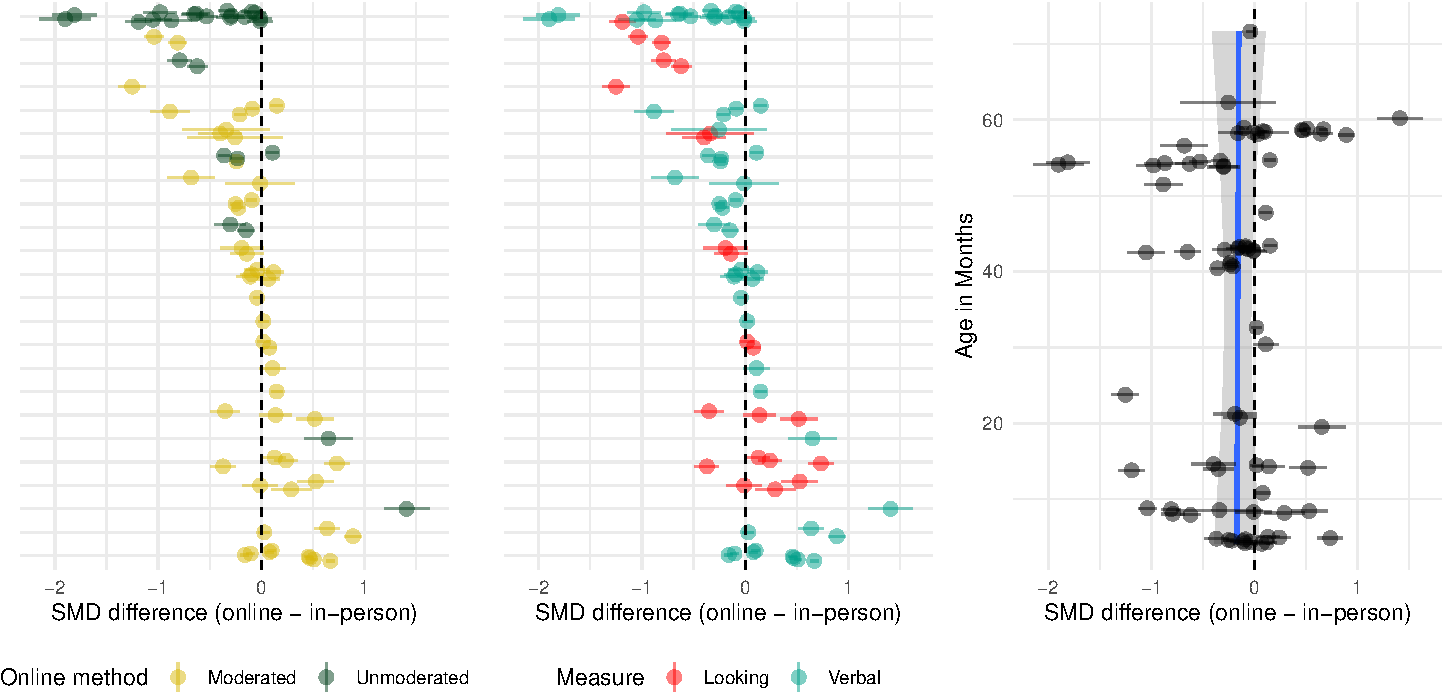
\includegraphics[width=1\linewidth]{OnlineMA_main_files/figure-latex/forest-1} 

}

\caption{Forest plots of studies. Each dot is the difference between and in-person measure and a corresponding online measure. In left and center plots, each row is one study (paper or pair of papers). On right plot, y-axis is the average age of the children in the two samples being compared.}\label{fig:forest}
\end{figure}

\begin{table}[!h]

\caption{\label{tab:coeffs}Table of coefficients for the pre-registered models. The overall model is shown first, followed by the three models with moderators.}
\centering
\begin{tabular}[t]{lrlr}
\toprule
Coefficient & Estimate & 95\% CI & P-value\\
\midrule
\addlinespace[0.3em]
\multicolumn{4}{l}{\textbf{Overall}}\\
\hspace{1em}Intercept & 0.84 & {}[0.46, 1.21] & 0.000\\
\hspace{1em}online & -0.15 & {}[-0.38, 0.08] & 0.210\\
\addlinespace[0.3em]
\multicolumn{4}{l}{\textbf{Looking v Verbal}}\\
\hspace{1em}Intercept & 0.73 & {}[0.42, 1.04] & 0.000\\
\hspace{1em}online & -0.29 & {}[-0.7, 0.11] & 0.155\\
\hspace{1em}verbal & -0.06 & {}[-0.43, 0.31] & 0.745\\
\hspace{1em}online:verbal & 0.23 & {}[-0.27, 0.72] & 0.375\\
\addlinespace[0.3em]
\multicolumn{4}{l}{\textbf{Age}}\\
\hspace{1em}Intercept & 0.68 & {}[0.51, 0.86] & 0.000\\
\hspace{1em}online & -0.14 & {}[-0.38, 0.1] & 0.244\\
\hspace{1em}age\_centered\_mo & 0.00 & {}[-0.01, 0.01] & 0.731\\
\hspace{1em}online:age\_centered\_mo & 0.01 & {}[-0.01, 0.02] & 0.342\\
\addlinespace[0.3em]
\multicolumn{4}{l}{\textbf{Moderated v Un-moderated}}\\
\hspace{1em}Intercept & 0.69 & {}[0.52, 0.86] & 0.000\\
\hspace{1em}online & -0.19 & {}[-0.45, 0.07] & 0.151\\
\hspace{1em}unmoderated & 0.13 & {}[-0.22, 0.48] & 0.461\\
\bottomrule
\end{tabular}
\end{table}

\hypertarget{confirmatory-analysis}{%
\subsection{Confirmatory Analysis}\label{confirmatory-analysis}}

Overall, the meta-analysis estimated a small negative, non-significant effect of online study modality, Est=-0.15, 95\% CI={[}-0.38, 0.08{]}, p=0.21. Additionally, we did not find any significant effect of our preregistered moderators or any significant interactions between the moderators and study modality. See Table \ref{tab:coeffs} for coefficient values. Figure \ref{fig:forest} shows the effect size differences of experiments by moderators.

\hypertarget{exploratory-analysis}{%
\subsection{Exploratory Analysis}\label{exploratory-analysis}}

\begin{longtable}[]{@{}lllr@{}}
\caption{\label{tab:ecoeffs}Mean SMD by study modality, data-collection method, and type of dependent measure}\tabularnewline
\toprule()
Modality & Method & Measure & SMD \\
\midrule()
\endfirsthead
\toprule()
Modality & Method & Measure & SMD \\
\midrule()
\endhead
in-person & moderated & looking & 0.091 \\
in-person & moderated & verbal & 0.063 \\
online & moderated & looking & 0.068 \\
online & moderated & verbal & 0.041 \\
online & unmoderated & looking & 0.021 \\
online & unmoderated & verbal & 0.062 \\
\bottomrule()
\end{longtable}

We also examined which combinations of methods and measures tended to yield the strongest and weakest effect sizes relative to their in-person counterparts. Although our model is likely underpowered to detect significant interactions between study modality, data-collection method, and dependent measure, unmoderated studies with looking measures yielded the noticeably weakest effect sizes compared to their in-person counterparts, an average difference of 0.07 (See Table \ref{tab:ecoeffs}).

\begin{figure}[h]

{\centering 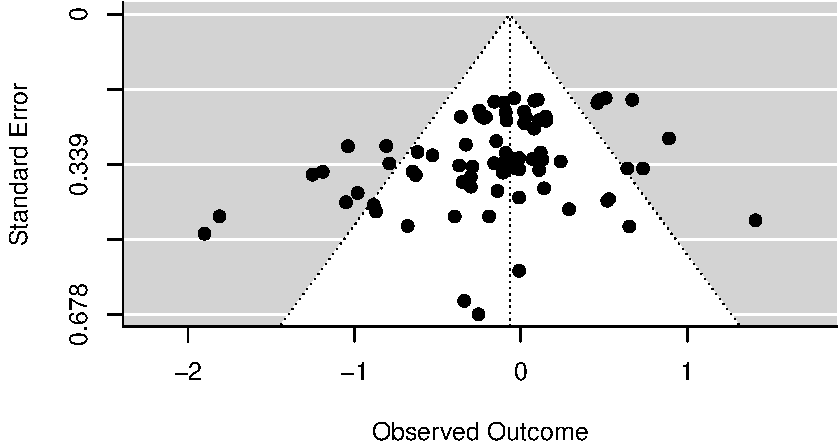
\includegraphics[width=0.8\linewidth]{OnlineMA_main_files/figure-latex/funnel-1} 

}

\caption{Funnel plot of the differences in effect size between pairs of in-person and online studies. A positive observed outcome means the online study had a large effect. \label{funnel}}\label{fig:funnel}
\end{figure}

Additionally, we conducted an exploratory analysis of potential publication bias. It was unclear how we might expect publication biases to manifest themselves, given that there is some possibility of notoriety for either showing \emph{or} failing to show differences between online and in-person testing.

We analyzed publication bias in the differences in effect sizes between each online and in-lab pair of samples. This analysis checks for publication bias on the basis of whether online studies match the results of the in-person studies. For each online and in-person pair on the same study, we calculated a standard mean difference in effect size between the two studies as well as the variance of this difference. The resulting funnel plot is shown in Figure \ref{fig:funnel}. According to Egger's regression test for funnel plot asymmetry, this plot is asymmetric (p=0.00) and the limit estimate of the effect as standard error goes to zero is 0.37 {[}0.01, 0.72{]}. Overall, we found no clear bias to publish papers with either larger or smaller differences in effect size than expected.

\hypertarget{discussion}{%
\section{Discussion}\label{discussion}}

By aggregating across a growing literature of online studies, the current meta-analysis provides a birds-eye view of how developmental studies traditionally conducted in-person fare compared to closely matched counterparts conducted online. Our results suggest that overall, the results of online studies are comparable to those conducted in-person. Based on our analysis, the method of online data collection, type of dependent measure, and participant age did not appear to have a significant impact either. Nonetheless, the relatively small sample size limits our ability to make sweeping generalizations about any of our moderators, so future analysis is needed to determine the moderating effect, if any, that these factors exercise on the outcome of developmental studies conducted online.

It is also important to consider additional factors that could influence these results or the way we interpret them. Chiefly, the current analysis is quite coarse-grained and considers one particular dichotomy within study modality: in-person vs online. Yet, there are many ways that developmental studies can be further subdivided. For example, studies are conducted both in quiet spaces (e.g., in lab, at home) and loud spaces (e.g., parks, museums). Therefore, online studies might out- or underperform studies conducted in particular in-person locations. Our moderators are also correspondingly course-grained, particularly dependent measure (looking vs verbal). Qualitatively, unmoderated studies with looking measures had the smallest effect sizes relative to their in-person counterparts. However, smaller effect sizes online could reflect true non-replications of the in-person results rather than a lack of online studies' sensitivity. Because our small sample size renders our analysis underpowered to detect weaker effects of moderators, our the current results and their interpretation are subject to change as online methods improve and comparisons to in-person studies are better understood.

Although developmental researchers have had decades of experience designing and running experiments in-person, most have only had a few years or less of experience developing online studies. Thus, our meta-analysis might underestimate the effectiveness of online studies due to researcher and experimenter inexperience. Over the next several years, as developmental researchers develop expertise and experience with online studies, effect sizes might increase for any number of reasons, including better experimenter-participant interactions, better stimulus design, and more accurate methods of measurements (i.e., automatic looking time measures, see Erel et al., 2022). Relatedly, as new methods are developed and adapted for online experiments, researchers should not take the current findings as a blanket declaration that all online studies produce comparable results to their in-person counterparts; some might underperform, while others might outperform. Nonetheless, the current results suggest that across currently employed developmental methodologies, studies conducted with children online are generally comparable to those conducted in-person.

The composition of our sample might also bias our results. To match online and in-person methods as closely as possible, we only considered direct online replications for the current meta-analysis. While this approach ensures that data were collected online and in-person using similar methods and procedures, it limits our sample size and may bias our sample. For example, perhaps researchers disproportionately choose to conduct online replications of strong or well-established effects rather than replicate more subtle, weaker effects. Nonetheless, our analysis found no significant publication bias in terms of favoring stronger online effect sizes or non-replications among the studies we sampled. We also included an open call for unpublished data in an attempt to limit the file drawer problem (see Rosenthal, 1979). Of the published and unpublished online replications that were available to include in our sample, we found comparable effect sizes online (compared to in-person); however, researchers should exercise caution as this sample may not be representative for their particular questions of interest.

\hypertarget{conclusion}{%
\section{Conclusion}\label{conclusion}}

Although online data collection precludes certain research methodologies or measures (e.g., exploration of a physical environment), the general similarity in outcomes for in-person and online studies with children paint an optimistic picture for online developmental research going forward. However, beyond enabling the collection of high quality, low cost data, online research also stands to benefit the broader scientific community as a whole. Conducting studies online allows researchers to sample beyond the local community surrounding their home institution. And importantly, for many online participants, an online study with a developmental researcher is their first interaction with a scientist. As online research expands among developmental researchers, we are presented with an unprecedented outreach opportunity to directly interact more closely with those we hope our research will allow us to better understand and help -- parents and children.

\newpage

\hypertarget{references}{%
\section{References}\label{references}}

\hypertarget{refs}{}
\begin{CSLReferences}{1}{0}
\leavevmode\vadjust pre{\hypertarget{ref-aboody2022says}{}}%
\textsuperscript{*} Aboody, R., Yousif, S. R., Sheskin, M., \& Keil, F. C. (2022). Says who? Children consider informants' sources when deciding whom to believe. \emph{Journal of Experimental Psychology: General}.

\leavevmode\vadjust pre{\hypertarget{ref-banki2022comparing}{}}%
\textsuperscript{*} Bánki, A., Eccher, M. de, Falschlehner, L., Hoehl, S., \& Markova, G. (2022). Comparing online webcam-and laboratory-based eye-tracking for the assessment of infants' audio-visual synchrony perception. \emph{Frontiers in Psychology}, 6162.

\leavevmode\vadjust pre{\hypertarget{ref-bochynska2021bringing}{}}%
\textsuperscript{*} Bochynska, A., \& Dillon, M. R. (2021). Bringing home baby euclid: Testing infants' basic shape discrimination online. \emph{Frontiers in Psychology}, 6002.

\leavevmode\vadjust pre{\hypertarget{ref-buhrmester2016amazon}{}}%
Buhrmester, M., Kwang, T., \& Gosling, S. D. (2016). \emph{Amazon's mechanical turk: A new source of inexpensive, yet high-quality data?}

\leavevmode\vadjust pre{\hypertarget{ref-bulgarelli2022talker}{}}%
Bulgarelli, F., \& Bergelson, E. (2022). Talker variability shapes early word representations in english-learning 8-month-olds. \emph{Infancy}, \emph{27}(2), 341--368.

\leavevmode\vadjust pre{\hypertarget{ref-chuey2021moderated}{}}%
\textsuperscript{*} Chuey, A., Asaba, M., Bridgers, S., Carrillo, B., Dietz, G., Garcia, T., et al.others. (2021). Moderated online data-collection for developmental research: Methods and replications. \emph{Frontiers in Psychology}, 4968.

\leavevmode\vadjust pre{\hypertarget{ref-chuey2020children}{}}%
Chuey, A., Lockhart, K., Sheskin, M., \& Keil, F. (2020). Children and adults selectively generalize mechanistic knowledge. \emph{Cognition}, \emph{199}, 104231.

\leavevmode\vadjust pre{\hypertarget{ref-chuey2021no}{}}%
Chuey, A., McCarthy, A., Lockhart, K., Trouche, E., Sheskin, M., \& Keil, F. (2021). No guts, no glory: Underestimating the benefits of providing children with mechanistic details. \emph{Npj Science of Learning}, \emph{6}(1), 1--7.

\leavevmode\vadjust pre{\hypertarget{ref-dejesus2021young}{}}%
DeJesus, J. M., Venkatesh, S., \& Kinzler, K. D. (2021). Young children's ability to make predictions about novel illnesses. \emph{Child Development}, \emph{92}(5), e817--e831.

\leavevmode\vadjust pre{\hypertarget{ref-dillon2020infants}{}}%
\textsuperscript{*} Dillon, M. R., Izard, V., \& Spelke, E. S. (2020). Infants' sensitivity to shape changes in 2D visual forms. \emph{Infancy}, \emph{25}(5), 618--639.

\leavevmode\vadjust pre{\hypertarget{ref-erel2022icatcher}{}}%
Erel, Y., Potter, C. E., Jaffe-Dax, S., Lew-Williams, C., \& Bermano, A. H. (2022). iCatcher: A neural network approach for automated coding of young children's eye movements. \emph{Infancy}, \emph{27}(4), 765--779.

\leavevmode\vadjust pre{\hypertarget{ref-escudero2021four}{}}%
\textsuperscript{*} Escudero, P., Pino Escobar, G., Casey, C. G., \& Sommer, K. (2021). Four-year-old's online versus face-to-face word learning via eBooks. \emph{Frontiers in Psychology}, 450.

\leavevmode\vadjust pre{\hypertarget{ref-fenson1994variability}{}}%
Fenson, L., Dale, P. S., Reznick, J. S., Bates, E., Thal, D. J., Pethick, S. J., \ldots{} Stiles, J. (1994). Variability in early communicative development. \emph{Monographs of the Society for Research in Child Development}, i--185.

\leavevmode\vadjust pre{\hypertarget{ref-gasparini2022online}{}}%
Gasparini, C., Caravale, B., Focaroli, V., Paoletti, M., Pecora, G., Bellagamba, F., \ldots{} Addessi, E. (2022). Online assessment of motor, cognitive, and communicative achievements in 4-month-old infants. \emph{Children}, \emph{9}(3), 424.

\leavevmode\vadjust pre{\hypertarget{ref-gerard2022extragrammaticality}{}}%
\textsuperscript{*} Gerard, J. (2022). The extragrammaticality of the acquisition of adjunct control. \emph{Language Acquisition}, \emph{29}(2), 107--134.

\leavevmode\vadjust pre{\hypertarget{ref-hamlin2015case}{}}%
\textsuperscript{*} Hamlin, J. (2015). The case for social evaluation in preverbal infants: Gazing toward one's goal drives infants' preferences for helpers over hinderers in the hill paradigm. \emph{Frontiers in Psychology}, \emph{5}, 1563.

\leavevmode\vadjust pre{\hypertarget{ref-kidd2022diverse}{}}%
Kidd, E., \& Garcia, R. (2022). How diverse is child language acquisition research? \emph{First Language}, 01427237211066405.

\leavevmode\vadjust pre{\hypertarget{ref-kominsky2021there}{}}%
\textsuperscript{*} Kominsky, J. F., Shafto, P., \& Bonawitz, E. (2021). {``There's something inside''}: Children's intuitions about animate agents. \emph{PloS One}, \emph{16}(5), e0251081.

\leavevmode\vadjust pre{\hypertarget{ref-lapidow2021tale}{}}%
\textsuperscript{*} Lapidow, E., Tandon, T., Goddu, M., \& Walker, C. M. (2021). A tale of three platforms: Investigating preschoolers' second-order inferences using in-person, zoom, and lookit methodologies. \emph{Frontiers in Psychology}, \emph{12}, 731404.

\leavevmode\vadjust pre{\hypertarget{ref-lo2021tablet}{}}%
Lo, C. H., Rosslund, A., Chai, J. H., Mayor, J., \& Kartushina, N. (2021). Tablet assessment of word comprehension reveals coarse word representations in 18--20-month-old toddlers. \emph{Infancy}, \emph{26}(4), 596--616.

\leavevmode\vadjust pre{\hypertarget{ref-lourenco2020no}{}}%
Lourenco, S. F., \& Tasimi, A. (2020). No participant left behind: Conducting science during COVID-19. \emph{Trends in Cognitive Sciences}, \emph{24}(8), 583--584.

\leavevmode\vadjust pre{\hypertarget{ref-margoni2018infants}{}}%
\textsuperscript{*} Margoni, F., Baillargeon, R., \& Surian, L. (2018). Infants distinguish between leaders and bullies. \emph{Proceedings of the National Academy of Sciences}, \emph{115}(38), E8835--E8843.

\leavevmode\vadjust pre{\hypertarget{ref-moher2015preferred}{}}%
Moher, D., Shamseer, L., Clarke, M., Ghersi, D., Liberati, A., Petticrew, M., \ldots{} Stewart, L. A. (2015). Preferred reporting items for systematic review and meta-analysis protocols (PRISMA-p) 2015 statement. \emph{Systematic Reviews}, \emph{4}(1), 1--9.

\leavevmode\vadjust pre{\hypertarget{ref-morini2021webcams}{}}%
\textsuperscript{*} Morini, G., \& Blair, M. (2021). Webcams, songs, and vocabulary learning: A comparison of in-person and remote data collection as a way of moving forward with child-language research. \emph{Frontiers in Psychology}, 3347.

\leavevmode\vadjust pre{\hypertarget{ref-nelson2021comparing}{}}%
\textsuperscript{*} Nelson, P. M., Scheiber, F., Laughlin, H. M., \& Demir-Lira, Ö. (2021). Comparing face-to-face and online data collection methods in preterm and full-term children: An exploratory study. \emph{Frontiers in Psychology}, 5025.

\leavevmode\vadjust pre{\hypertarget{ref-nielsen2017persistent}{}}%
Nielsen, M., Haun, D., Kärtner, J., \& Legare, C. H. (2017). The persistent sampling bias in developmental psychology: A call to action. \emph{Journal of Experimental Child Psychology}, \emph{162}, 31--38.

\leavevmode\vadjust pre{\hypertarget{ref-pasquini2007preschoolers}{}}%
\textsuperscript{*} Pasquini, E. S., Corriveau, K. H., Koenig, M., \& Harris, P. L. (2007). Preschoolers monitor the relative accuracy of informants. \emph{Developmental Psychology}, \emph{43}(5), 1216.

\leavevmode\vadjust pre{\hypertarget{ref-rhodes2020advancing}{}}%
Rhodes, M., Rizzo, M. T., Foster-Hanson, E., Moty, K., Leshin, R. A., Wang, M., \ldots{} Ocampo, J. D. (2020). Advancing developmental science via unmoderated remote research with children. \emph{Journal of Cognition and Development}, \emph{21}(4), 477--493.

\leavevmode\vadjust pre{\hypertarget{ref-rosenthal1979file}{}}%
Rosenthal, R. (1979). The file drawer problem and tolerance for null results. \emph{Psychological Bulletin}, \emph{86}(3), 638.

\leavevmode\vadjust pre{\hypertarget{ref-schidelko2021online}{}}%
\textsuperscript{*} Schidelko, L. P., Schünemann, B., Rakoczy, H., \& Proft, M. (2021). Online testing yields the same results as lab testing: A validation study with the false belief task. \emph{Frontiers in Psychology}, 4573.

\leavevmode\vadjust pre{\hypertarget{ref-scott2017lookitB}{}}%
\textsuperscript{*} Scott, K., Chu, J., \& Schulz, L. (2017). Lookit (part 2): Assessing the viability of online developmental research, results from three case studies. \emph{Open Mind}, \emph{1}(1), 15--29.

\leavevmode\vadjust pre{\hypertarget{ref-scott2017lookit}{}}%
Scott, K., \& Schulz, L. (2017). Lookit (part 1): A new online platform for developmental research. \emph{Open Mind}, \emph{1}(1), 4--14.

\leavevmode\vadjust pre{\hypertarget{ref-sheskin2018thechildlab}{}}%
Sheskin, M., \& Keil, F. (2018). \emph{TheChildLab. Com a video chat platform for developmental research}.

\leavevmode\vadjust pre{\hypertarget{ref-sheskin2020online}{}}%
Sheskin, M., Scott, K., Mills, C. M., Bergelson, E., Bonawitz, E., Spelke, E. S., et al.others. (2020). Online developmental science to foster innovation, access, and impact. \emph{Trends in Cognitive Sciences}, \emph{24}(9), 675--678.

\leavevmode\vadjust pre{\hypertarget{ref-silver2021measuring}{}}%
\textsuperscript{*} Silver, A. M., Elliott, L., Braham, E. J., Bachman, H. J., Votruba-Drzal, E., Tamis-LeMonda, C. S., \ldots{} Libertus, M. E. (2021). Measuring emerging number knowledge in toddlers. \emph{Frontiers in Psychology}, 3057.

\leavevmode\vadjust pre{\hypertarget{ref-skerry2014preverbal}{}}%
\textsuperscript{*} Skerry, A. E., \& Spelke, E. S. (2014). Preverbal infants identify emotional reactions that are incongruent with goal outcomes. \emph{Cognition}, \emph{130}(2), 204--216.

\leavevmode\vadjust pre{\hypertarget{ref-smith-flores2022}{}}%
Smith-Flores, A. S., Perez, J., Zhang, M. H., \& Feigenson, L. (2022b). Online measures of looking and learning in infancy. \emph{Infancy}, \emph{27}(1), 4--24.

\leavevmode\vadjust pre{\hypertarget{ref-smith2022online}{}}%
Smith-Flores, A. S., Perez, J., Zhang, M. H., \& Feigenson, L. (2022a). Online measures of looking and learning in infancy. \emph{Infancy}, \emph{27}(1), 4--24.

\leavevmode\vadjust pre{\hypertarget{ref-stahl2015observing}{}}%
Stahl, A. E., \& Feigenson, L. (2015). Observing the unexpected enhances infants' learning and exploration. \emph{Science}, \emph{348}(6230), 91--94.

\leavevmode\vadjust pre{\hypertarget{ref-teglas2007intuitions}{}}%
\textsuperscript{*} Téglás, E., Girotto, V., Gonzalez, M., \& Bonatti, L. L. (2007). Intuitions of probabilities shape expectations about the future at 12 months and beyond. \emph{Proceedings of the National Academy of Sciences}, \emph{104}(48), 19156--19159.

\leavevmode\vadjust pre{\hypertarget{ref-yuen2022}{}}%
\textsuperscript{*} todo, todo. (2022a). \emph{Todo}.

\leavevmode\vadjust pre{\hypertarget{ref-mani2022}{}}%
\textsuperscript{*} todo, todo. (2022b). \emph{Todo}.

\leavevmode\vadjust pre{\hypertarget{ref-vales2021research}{}}%
\textsuperscript{*} Vales, C., Wu, C., Torrance, J., Shannon, H., States, S. L., \& Fisher, A. V. (2021). Research at a distance: Replicating semantic differentiation effects using remote data collection with children participants. \emph{Frontiers in Psychology}, \emph{12}, 697550.

\leavevmode\vadjust pre{\hypertarget{ref-viechtbauer2010conducting}{}}%
Viechtbauer, W. (2010). Conducting meta-analyses in r with the metafor package. \emph{Journal of Statistical Software}, \emph{36}(3), 1--48.

\leavevmode\vadjust pre{\hypertarget{ref-yoon2019preschool}{}}%
\textsuperscript{*} Yoon, E. J., \& Frank, M. C. (2019). Preschool children's understanding of polite requests. \emph{CogSci}, 3179--3185.

\end{CSLReferences}


\end{document}
